\section{System and Research-Loop Architecture}
\label{sec:system}

The programme's second contribution is architectural: the research loop that produced the results is itself a released, replayable system. Figure~\ref{fig:architecture} shows the three tiers.

\begin{figure}[t]
\centering
\resizebox{\columnwidth}{!}{% Hand-authored TikZ. System architecture: controller-actuator-plant with the
% auto-research loop. Structure mirrors src/prabodha/ modules and the EFE
% selector in src/prabodha/efe/ (see Appendix on module map).
\begin{tikzpicture}[
  font=\scriptsize,
  box/.style={draw, rounded corners=2pt, align=center, inner sep=4pt, minimum height=18pt},
  plant/.style={box, fill=gray!12, minimum width=88pt},
  act/.style={box, fill=blue!12, minimum width=88pt},
  ctrl/.style={box, fill=orange!15, minimum width=88pt},
  loop/.style={box, fill=teal!10, minimum width=100pt},
  arr/.style={-{Latex[length=5pt]}, thick},
  lbl/.style={font=\tiny, midway, fill=white, inner sep=1pt},
]
% plant
\node[plant] (plant) at (0,0) {frozen decoder LLM\\residual stream, workspace band};
% actuator column
\node[act] (writer) at (-2.6,1.7) {writer\\$h \leftarrow h + \alpha\, J^{\top}u$};
\node[act] (lens) at (2.6,1.7) {band-targeted lens\\readback $J_{\ell} h \to$ tokens};
% controller
\node[ctrl] (timing) at (-2.6,3.3) {timing gate\\write iff $H_t > \tau$};
\node[ctrl] (verify) at (2.6,3.3) {verifier\\readback vs.\ intent};
\node[ctrl] (budget) at (0,4.4) {budget monitor\\$|\overline{\Delta H}| \le 0.5$ nats};
% research loop
\node[loop] (menu) at (-2.6,6.0) {registered menu\\candidate experiments};
\node[loop] (efe) at (0,7.1) {EFE selector\\$\arg\max\ \mathcal{G}$ over candidates};
\node[loop] (gate) at (2.6,6.0) {dual-closure gate\\code gate $\wedge$ domain gate};
\node[loop, fill=red!8] (review) at (0,5.2) {adversarial review\\isolated agent, gate brief only};
% wiring: control loop
\draw[arr] (timing) -- (writer) node[lbl] {permit};
\draw[arr] (writer) -- (plant) node[lbl] {band write};
\draw[arr] (plant) -- (lens) node[lbl] {band state};
\draw[arr] (lens) -- (verify) node[lbl] {read-out};
\draw[arr] (plant.north) to[bend left=12] node[lbl] {step entropy $H_t$} (timing.south east);
\draw[arr] (verify) -- (budget);
\draw[arr] (timing) -- (budget);
% wiring: research loop
\draw[arr] (efe) -- (menu) node[lbl] {select};
\draw[arr] (menu.south) to[bend right=18] node[lbl] {dispatch} (budget.west);
\draw[arr] (budget.east) to[bend right=18] node[lbl] {evidence} (gate.south);
\draw[arr] (gate) -- (efe) node[lbl] {verdict $\to$ belief};
\draw[arr] (gate) -- (review);
\draw[arr] (review) -- (efe) node[lbl] {corrections};
% ledgers
\node[box, fill=yellow!12, minimum width=70pt] (ledger) at (3.4,7.6) {ledgers\\gates/*.json, efe\_ledger.jsonl};
\draw[arr, dashed] (gate) -- (ledger);
\draw[arr, dashed] (efe) -- (ledger);
% braces
\node[font=\tiny, rotate=90, gray] at (-4.4,1.0) {plant + actuator};
\node[font=\tiny, rotate=90, gray] at (-4.4,3.8) {controller (doctrine)};
\node[font=\tiny, rotate=90, gray] at (-4.4,6.4) {auto-research loop};
\end{tikzpicture}
}
\caption{System architecture. Lower tier: the frozen plant with its actuator pair, transported writes (Equation~\ref{eq:write}) and band-targeted lens readback. Middle tier: the doctrine as controller, an entropy timing gate, a readback verifier, and a budget monitor. Upper tier: the auto-research loop, in which an expected-free-energy selector chooses the next experiment from a registered menu, results close through dual gates, and isolated adversarial reviews feed corrections back. All state flows through committed ledgers.}
\label{fig:architecture}
\end{figure}

\subsection{Control Loop}

At each decode step the controller receives the step entropy $H_t$, permits a write when $H_t > \tau$ and the budget monitor projects the trajectory-average entropy change to remain inside $\pm0.5$ nats, and applies Equation~\ref{eq:write} at the band. The verifier periodically reads the band through the band-targeted lens and scores the read-out against the intended concept. Timing, amplitude, band membership, and budget are configuration, not code: every tunable lives in a versioned YAML file validated by typed schemas, so a gate record plus a configuration file reproduces a run exactly.

\subsection{Dual-Closure Gates}

A research loop closes only when two independent gates pass. The code gate requires the test suite and static analysis to be green. The domain gate evaluates the pre-registered scientific criterion for the loop, stated before dispatch with seeds, commands, and thresholds, and issues pass, fail, or fail-on-margin with the raw evidence embedded in the record. The two gates are deliberately non-fungible: several loops in the ledger have passing code gates and failing domain gates (L1, L2, L3, L4, L17, L21), and these closed as registered negative results rather than being re-run to a pass. Each gate record also carries an amendment log; retroactive corrections, such as the sampling-stream repair described below, are visible as amendments rather than silent edits.

\subsection{Expected-Free-Energy Experiment Selection}

Candidate experiments are registered in menus, each candidate carrying an expected information gain, a preference weight, a compute cost, and a tier (smoke, screen, or confirm, with escalating seed and sample requirements). The selector scores candidates by expected free energy, dispatches the maximiser, observes the resulting gate verdict, and updates its beliefs; beliefs replay deterministically from the ledger of past verdicts, so the entire programme's decision sequence can be re-derived from committed artifacts. Over the programme the selector consumed nine menus in twenty-seven cycles, and its ledger records 267 observation events, 41 proposals, and 27 spend entries. Two formally logged divergences, cases where new evidence superseded an earlier point estimate, were resolved by registered supersession rather than deletion (Appendix~\ref{app:efe}). Contradictions between engineering requirements (steering strength against freedom cost, rigour against velocity, GPU productivity against co-resident job safety) were worked through a TRIZ contradiction log before implementation \cite{Altshuller1984}; the log is released with the repository.

\subsection{Adversarial Review}

Eighteen reviews were performed by isolated agents given only gate records and contracts, without access to the working tree or the researcher's narrative. Reviews returned verdicts of the form merge-with-corrections, and every correction was applied and committed before the affected loop closed. Material catches include: a cost-model miscalibration in the selector; a ledger-replay bug; the discovery that a single per-run random seed correlated all forty generations within an arm, which invalidated the effective sample size of every earlier sampling estimate and forced per-generation seeding derived from a hash of seed, arm, concept, and stub (the stream fix, gate L9); a candidate name that overclaimed a robustness result (L17); the formal supersession of stale dose-response levels after the stream fix (L18, L19); and the withdrawal of an independence claim that a review showed to be a deterministic replay artifact rather than a replication (L19). Appendix~\ref{app:reviews} catalogues all eighteen.

\subsection{Compute Discipline}

All experiments ran on a single shared DGX Spark node (GB10, unified-memory aarch64) co-resident with unrelated training jobs. A guard script gates every dispatch on GPU idleness, per-loop budget, and a kill-switch file; contention events are recorded in gate metadata. The full programme consumed 18.17 GPU-hours across nineteen budgeted loops (Figure~\ref{fig:compute}), a figure reported to make the cost of the evidence auditable.

\begin{figure}[t]
\centering
\resizebox{\columnwidth}{!}{% Auto-generated from committed gate JSONs by generate_figures.py. Do not edit by hand.

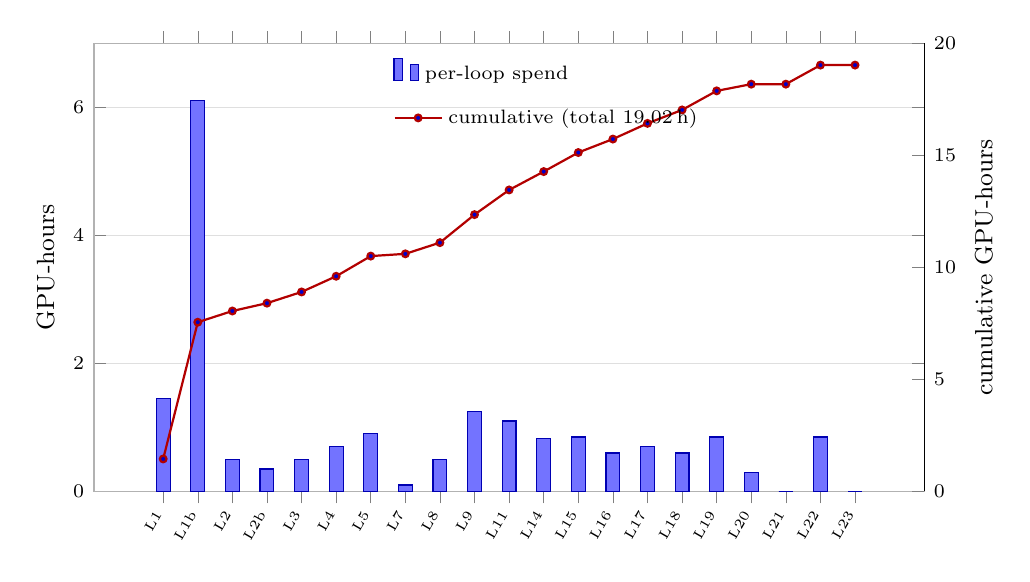
\begin{tikzpicture}
\begin{axis}[
  width=\columnwidth, height=0.6\columnwidth,
  ybar, /pgf/bar width=5pt,
  symbolic x coords={L1,L1b,L2,L2b,L3,L4,L5,L7,L8,L9,L11,L14,L15,L16,L17,L18,L19,L20,L21,L22,L23},
  xtick=data, x tick label style={rotate=60, anchor=east, font=\tiny},
  ymin=0, ymax=7, ylabel={GPU-hours},
  label style={font=\small}, tick label style={font=\scriptsize},
  legend style={font=\scriptsize, at={(0.35,0.98)}, anchor=north west, draw=none, fill=none},
  ymajorgrids, grid style={gray!25}, axis line style={gray!60},
]
\addplot+[fill=blue!55, draw=blue!70!black] coordinates {(L1,1.45) (L1b,6.1) (L2,0.5) (L2b,0.35) (L3,0.5) (L4,0.7) (L5,0.9) (L7,0.1) (L8,0.5) (L9,1.25) (L11,1.1) (L14,0.82) (L15,0.85) (L16,0.6) (L17,0.7) (L18,0.6) (L19,0.85) (L20,0.3) (L21,0.0) (L22,0.85) (L23,0)};
\addlegendentry{per-loop spend}
\end{axis}
\begin{axis}[
  width=\columnwidth, height=0.6\columnwidth,
  symbolic x coords={L1,L1b,L2,L2b,L3,L4,L5,L7,L8,L9,L11,L14,L15,L16,L17,L18,L19,L20,L21,L22,L23}, xtick=\empty,
  ymin=0, ymax=20, axis y line*=right, axis x line=none,
  ylabel={cumulative GPU-hours}, ylabel near ticks,
  label style={font=\small}, tick label style={font=\scriptsize},
  legend style={font=\scriptsize, at={(0.35,0.88)}, anchor=north west, draw=none, fill=none},
]
\addplot+[red!70!black, thick, mark=*, mark size=1.2pt] coordinates {(L1,1.45) (L1b,7.55) (L2,8.05) (L2b,8.40) (L3,8.90) (L4,9.60) (L5,10.50) (L7,10.60) (L8,11.10) (L9,12.35) (L11,13.45) (L14,14.27) (L15,15.12) (L16,15.72) (L17,16.42) (L18,17.02) (L19,17.87) (L20,18.17) (L21,18.17) (L22,19.02) (L23,19.02)};
\addlegendentry{cumulative (total 19.02\,h)}
\end{axis}
\end{tikzpicture}
}
\caption{Compute ledger. Bars give per-loop GPU-hours as recorded in the programme state file; the line gives the cumulative total (18.17 GPU-hours). The largest single item is the 27B loadability replication (L1b, 6.1 h).}
\label{fig:compute}
\end{figure}
